\documentclass[14pt, fleqn, xcolor={dvipsnames, table}]{beamer}
\usepackage[T2A]{fontenc}
\usepackage[utf8]{inputenc}
\usepackage[english,russian]{babel}
\usepackage{amssymb,amsfonts,amsmath,mathtext}
\usepackage{cite,enumerate,float,indentfirst}
\usepackage{cancel}
\usepackage{graphicx}
\usepackage{animate}

\usepackage{tikz}
% \usepackage{enumitem}
\usetikzlibrary{shadows}

% \usepackage{enumitem}
% \setitemize{label=\usebeamerfont*{itemize item}%
%   \usebeamercolor[fg]{itemize item}
%   \usebeamertemplate{itemize item}}

\graphicspath{{images/}}

\usetheme{Madrid}
\usecolortheme{seahorse}
\renewcommand{\CancelColor}{\color{red}}

\setbeamercolor{footline}{fg=Blue!50}
\setbeamertemplate{footline}{
  \leavevmode%
  \hbox{%
  \begin{beamercolorbox}[wd=.333333\paperwidth,ht=2.25ex,dp=1ex,center]{}%
    И. Кураленок
  \end{beamercolorbox}%
  \begin{beamercolorbox}[wd=.333333\paperwidth,ht=2.25ex,dp=1ex,center]{}%
    Санкт-Петербург, 2017
  \end{beamercolorbox}%
  \begin{beamercolorbox}[wd=.333333\paperwidth,ht=2.25ex,dp=1ex,right]{}%
  Стр. \insertframenumber{} из \inserttotalframenumber \hspace*{2ex}
  \end{beamercolorbox}}%
  \vskip0pt%
}
\newcommand\indentdisplays[1]{%
     \everydisplay{\addtolength\displayindent{#1}%
     \addtolength\displaywidth{-#1}}}
\newcommand{\itemi}{\item[\checkmark]}

\newenvironment{mydescription}[1]
  {\begin{list}{}%
   {\renewcommand\makelabel[1]{\color{blue}##1:\hfill}%
   \settowidth\labelwidth{\makelabel{#1}}%
   \setlength\leftmargin{\labelwidth}
   \addtolength\leftmargin{\labelsep}}}
  {\end{list}}

\title{Уменшение размерности: обзор\\\small{}}
\author[]{\small{%
И.~Куралёнок}}
\date{}
\begin{document}

\begin{frame}
\maketitle
\small
\begin{center}
\vspace{-60pt}
\normalsize
\vspace{80pt}
\footnotesize СПб, 2017
\end{center}
\end{frame}

\section{Содержание}
\section{Постановка задачи уменьшения размерности}
\subsection{Зачем нужно}
\begin{frame}{Зачем бороться с размерностью?}
\begin{enumerate}
  \item Наглядность: сложно смотреть на 100-мерное пространство
  \item Количество данных и надежно подбираемых параметров зависимы
  \item Экономим стоимость использования:
  \begin{itemize}
    \item вычислительные ресурсы на этапе обучения и/или использования;
    \item стоимость отдельного измерения.
  \end{itemize}
  \item Убрать шум
  % \item Гибкость в построении данных
\end{enumerate}
\end{frame}

\begin{frame}{Проклятье размерности}
\small
\emph{Что происходит с расстояниями когда размерность увеличивается?} \\
Проведем простой опыт: будем равномерно выбирать точки из кубика $[0, 1]^n \subset \mathbb{R}^n$. \\
Оказывается, что при увеличении $n$:
\begin{itemize}
  \item Точки все ближе “жмутся” к краю
  \item Углы между точками выравниваются
  \item Окрестности все чаще упираются в границы
  \item Для того, чтобы пространство было плотным надо слишком много точек
\end{itemize}
$\Rightarrow$ Большая размерность — зло для kNN и не только для него!
\end{frame}

\subsection{Какие фичи бывают}
\begin{frame}{Постановка задачи обучения}{}
{\color{blue}С построением фичей}: повесим на клиента датчики \\
\textit{Наша цель повесить датчики правильно, зная какую информацию мы хотим получить.}\\
Похоже на glass box\\
~\\
{\color{blue}Без построения фичей}: льется поток неведомых данных \\
\textit{Хотим выделить сигналы, имеющие отношение к искомому} \\
Похоже на black box
\end{frame}

\subsection{Почему можно} % тут можно привести аналогию с каналом
\begin{frame}{Почему можно уменьшить размерность?}{В конструктивной постановке}
Датчики могут:
\begin{itemize}
  \item быть разные, а информация одна и та же;
  \item быть неудачно поставленны оператором и работать не так, как задумано.
\end{itemize}
\end{frame}

\begin{frame}{Почему можно уменьшить размерность?}{В случае сырых данных}
В случае сырых данных, мы по сути должны найти датчики, изучив их свойства по имеющимся данным. Поэтому все предыдущее верно и тут, а кроме этого:
\begin{itemize}
  \item надо понять где причина, а где следствие;
  \item отделить свойства передачи данных от информации.
\end{itemize}
\end{frame}

\subsection{Направления}
\begin{frame}{Как можно это делать}{}

{\color{blue}Feature selection (whitening)} \\
\textbf{Пример:} проверка стат гипотез, что фича нужна \\
\uncover<2->{\textbf{Девиз:} меньше фишек --- легче думать.} \\
~\\
{\color{blue}Feature extraction/construction (kostyl production)} \\
\textbf{Пример:} метод главных компонент (PCA) \\
\uncover<3->{\textbf{Девиз:} Мурзик, ну еще капельку!} \\
~\\
{\color{blue}Embedded models (velosiped prouction)}\\
\textbf{Пример:} LASSO \\
\uncover<4>{\textbf{Девиз:} само сдохнет.}
\end{frame}

\begin{frame}{Область применения}{Feature selection}
\textbf{Зачем:} оценка новых параметров, наглядность, экономия ресурсов, надежный подбор, прибрать шум. \\
\textbf{Когда:}
\begin{itemize}
  \item шум/сигнал (dB) у некоторых совсем поганый
  \item оценка источника сигнала
\end{itemize}
\end{frame}

\begin{frame}{Область применения}{Feature extraction}
\textbf{Зачем:} наглядность (быть аккуратными!), экономия ресурсов обучения и использования (предобработка), прибрать шум, гибкость в построении данных. \\
\textbf{Когда:}
\begin{itemize}
  \item несколько факторов про одно, но все глядят в разные стороны из-за особенностей реализации;
  \item хотим обобщающие факторы;
  \item понимаем структуру данных;
  \item хочется потратить время.
\end{itemize}
\end{frame}

\begin{frame}{Область применения}{Embedded models}
\textbf{Зачем:} экономия ресурсов использования, убрать шум \\
\textbf{Когда:}
\begin{itemize}
  \item ничего не знаем про данные, зато понимаем как может быть устроено хорошее решение;
  \item не хотим думать про механизм приемки фичей.
\end{itemize}
\end{frame}

\subsection{Какие есть теоретические ограничения}
\begin{frame}{Эффективная размерность}{Постановка задачи}
Бывают такие ситуации, когда размерность пространства задачи может быть явно меньше чем количество факторов.
\begin{center}
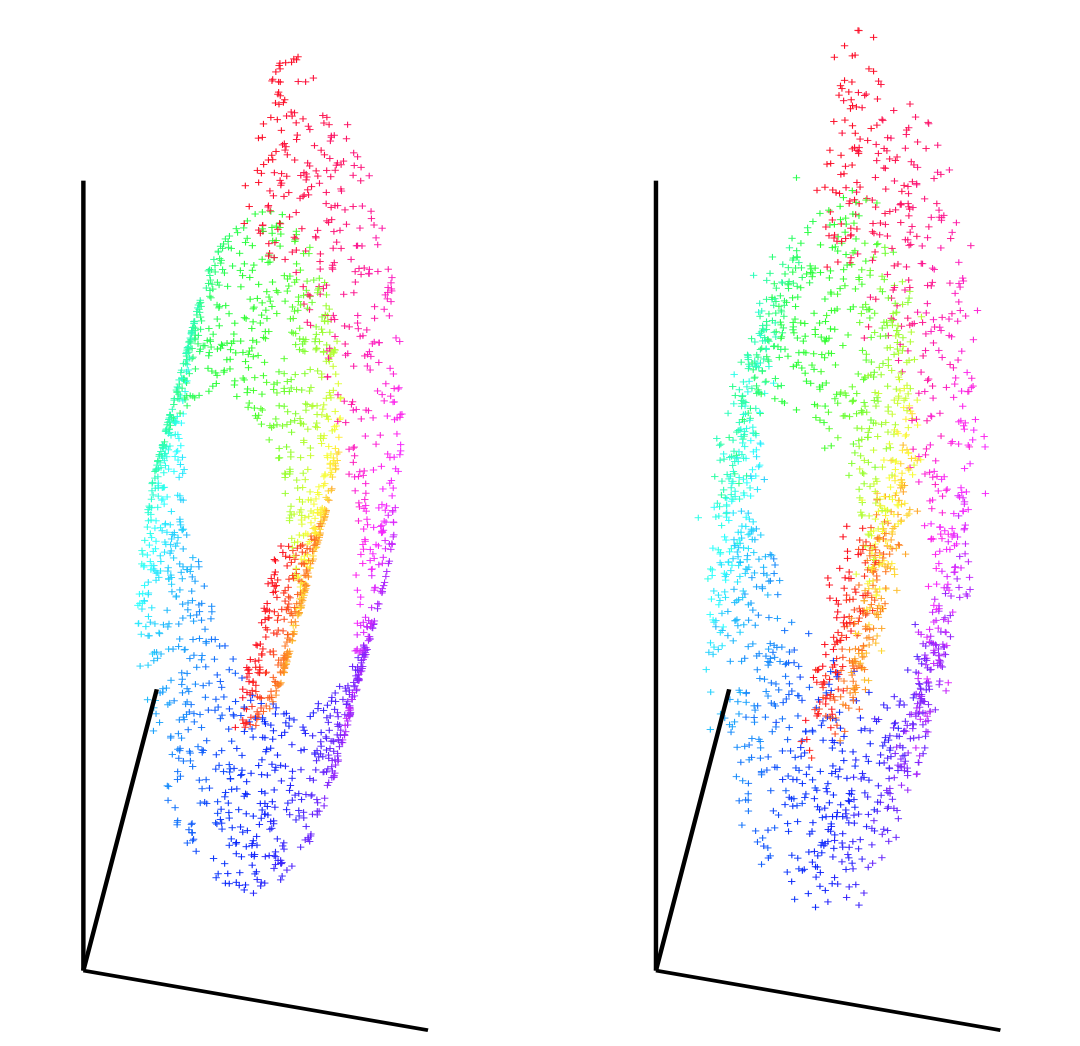
\includegraphics[width=0.4\textwidth]{swiss-roll.png}
\end{center}
\end{frame}
\begin{frame}{Эффективная размерность}{``Определение''}
\begin{definition}[Эффективная размерность]
Будем называть размерность $n' < n$ эффективной размерностью задачи, если существует такое преобразование пространства задачи в $\mathbb{R}^{n'}$, что сохраняет интересные нам свойства
\end{definition}
\end{frame}

\begin{frame}{Jonson-Lindestrauss lemma I}
\begin{theorem}{}
Для заданного $0<\epsilon<1$, множества точек $X \supset \mathbb{R}^{n\times m}$, числа $k > \frac{\log m}{\epsilon^2}$, существует линейное преобразование $f: \mathbb{R}^n \to \mathbb{R}^k$ такое, что:
$$
(1 - \epsilon) \|u - v\|_2^2 \le \|f(u) - f(v)\|_2^2 \le (1 + \epsilon) \|u - v\|_2^2
$$
для любой пары $(u,v) \in X^2$.
\end{theorem}
\end{frame}

\begin{frame}{Jonson-Lindestrauss lemma II}
К сожалению лемма довольно tight:
\begin{theorem}{}
Существует множество точек $X$, для которого потребуется $k = O(-\frac{\log m}{\epsilon^2 \log \epsilon})$.
\end{theorem}
Но мы помним:
\begin{itemize}
  \item ограничения только на линейные преобразования;
  \item есть предположение о полной информации, содержащейся в $X$.
\end{itemize}
\end{frame}

\begin{frame}{Как узнать эффективную размерность?}
\begin{itemize}
  \item Спектральная энтропия erank
  \item Сонаправленность соседей
  \item Измерение концентрации примеров вблизи точки
\end{itemize}
\end{frame}

\begin{frame}{SOM}{Самоорганизующиеся сети Кохоненна}
\textbf{Идея:} отобразить многомерное пространство в граф, зафиксированной структуры так, чтобы как можно лучше сохранить взаимные расстояния. \\
\textbf{Графы бывают разные:}
\begin{itemize}
  \item Простая 2/3-х мерная сеть
  \item Шестигранная сетка
  \item Односвязная “нить”.
\end{itemize}
\end{frame}

\begin{frame}{SOM}{процесс обучения}
Можно представить так: кидаем платок и расправляем его.
\begin{center}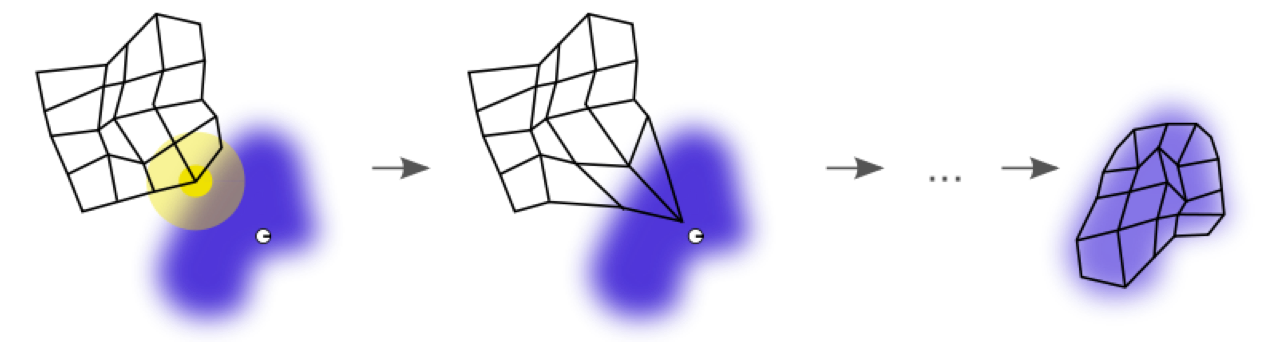
\includegraphics[width=0.7\textwidth]{SOM.png}\end{center}
\end{frame}

\begin{frame}{SOM}{алгоритм}
\textbf{Дано:} функция расстояния по графу ($G$), множество точек ($X \in \mathbb{R}^n$), дискаунт за расстояние ($q$), дискаунт за итерацию ($s$) 
\begin{enumerate}
  \item Инициализируем точки, соответствующие узлам графа $g_i$ в $\mathbb{R}^n$
  \item Выберем случайную точку $x^t$ в $X$
  \item Находим ближайший $g_{i_0}$
  \item ``Двигаем'' $g_i$ в сторону точки $x^t$, по принципу ``чем дальше, тем меньше'':
  $$
    g_i^{t+1} = g_i^t + q(G(i, i_0), t)s(t)(x_t - g_t)
  $$
  \item Переходим в п.2 пока не сошлось.
\end{enumerate}
\end{frame}

\begin{frame}{SOM}{свойства}
Что можно с их помощью делать:
\begin{itemize}
  \item Смотреть на данные ``глазами''
  \item Если из области следует какая-то структура, то можно подобрать ее распределение таким образом
  \item Аля PCA по 1D кривулинам, полученным с помощью SOM
\end{itemize}
Проблемы:
\begin{itemize}
  \item Результат существенно зависит от подбора начальных $g_i \Rightarrow$ зачастую не воспроизводим
  \item Никаких гарантий сходимости при $s(t) = 1$
  \item Никаких хороших математических свойств.
\end{itemize}
Но, it just works!
\end{frame}

\begin{frame}{SOM}{рекомендации SOMоводов}
\begin{itemize}
  \item Выбирать начальные значения не по рандому, а по PCA2
  \item Выбросить выбросы/сгладить движение от дистанции
  \item Бегать не в одном и том же порядке по множеству
  \item По минимуму использовать $s$.
\end{itemize}
\end{frame}

\section{Feature selection}
\begin{frame}{Feature selection}
Какие тут есть задачи?
\begin{itemize}
  \item Понять годится ли нам фича, или можно без нее:
  \begin{itemize}
    \item как это делать надежно;
    \item можно ли сделать подешевле.
  \end{itemize}
  \item Выбрать оптимальное подмножество факторов.
  \item Научиться строить модели, предпочитающие поменьше факторов.
\end{itemize}
\end{frame}

\subsection{Проверка полезности фичи}
\begin{frame}{Как можно понять нужна или нет фича?}
Можно проверить такую гипотезу:
\begin{theorem}{}{} \small Для множеств $X_B \in \mathbb{R}^{n\times m}$ и $X_T = (X_B, x) \in \mathbb{R}^{n\times (m+1)}$, парных последовательностей разбиений этих множеств:
$$\begin{array}{l}
\{(L_{Bt}, V_{Bt})\}_1^{\infty}, L_{Bt} \cup V_{Bt} = X_B, \forall t\\
\{(L_{Tt}, V_{Tt})\}_1^{\infty}, L_{Tt} \cup V_{Tt} = X_T, \forall t\\
\end{array}$$
, целевой функции $T(\beta, X)$ событие
$$
T(\arg \max_{\beta} T(L_{Bt}), V_{Bt}) \le T(\arg \max_{\beta} T(L_{Tt}), V_{Tt})
$$
выполняется с вероятностью не менее $1 - \alpha$.
\end{theorem}
\end{frame}

\begin{frame}{Немного о свойствах проверки}
\small
У подобной постановки есть несколько свойств:
\begin{itemize}
  \item сразу вставили повторную выборку, чтобы не париться;
  \item заметим, что подбираем прямо $\beta$, что означает зависимость метода от способа оптимизации;
  \item конкретный способ проверки подобной гипотезы зависит от распределения $T(\arg \max_{\beta} T(L_{Bt}), V_{Bt})$;
  \item считаем, что проверяемый фактор не влияет на это распределение;
  \item есть надежда на то, что исходный $X$ несмещен относительно генеральной совокупности по $T(\arg \max_{\beta} T(L_{Bt}), V_{Bt})$
  \item исходим из независимости $T(\arg \max_{\beta} T(L_{Bt}), V_{Bt})$ по $t$, что, конечно, не так :).
\end{itemize}
\end{frame}

\begin{frame}{Практическая реализация проверки}
Что нам нужно определить чтобы такое реализовать?
\begin{itemize}
  \item Понять как делить $X$.
  \item Выяснить какой критерий использовать.
  \item Найти необходимое количество разбиений для достижения уровня значимости $\alpha$.
  \item Нащупать границы применимости.
\end{itemize}
\end{frame}

\begin{frame}{Как делить $X$}{Мы делили апельсин...}
\small
Можно через BS, но мы побаиваемся зависимости, и делаем CV.\\
В CV обычно встает вопрос соотношения мощности $L$ и $V$. Есть две альтернативы:
\begin{itemize}
  \item Сделать $L$ поменьше \\
\uncover<2->{\footnotesize Увеличит variance $\beta$ и, соответственно, может повлиять на дисперсию случайных величин справа и слева, при фиксированном.}
  \item \small Сделать $T$ поменьше \\
\uncover<3->{\footnotesize Обычно мы строим $T$ используя информацию о независимости наблюдаемых точек, что приводит к обратной зависимости дисперсии от количества точек.}
\end{itemize}
$$
T(\arg \max_{\beta} T(L_{Bt}), V_{Bt}) \le T(\arg \max_{\beta} T(L_{Tt}), V_{Tt})
$$
\uncover<3->{$\Rightarrow$ надо найти баланс при котором достигается $\min var(T(\arg \max_{\beta} T(L_{Bt}), V_{Bt})$) }
\end{frame}

\begin{frame}{Какой критерий выбрать?}{}
Зависит от метода:
\begin{center}
\includegraphics[width=0.6\textwidth]{iterations.png}
\end{center}
Можно не париться и взять $WX$-тест, который работает почти всегда. 
\end{frame}

\begin{frame}{Сколько разбиений достаточно?}
\small
Само по себе значение статистики является случайной величиной со своей дисперсией, это надо учитывать.
\begin{center}
\includegraphics[width=0.6\textwidth]{wxvalues.png}
\end{center}
Зависит дисперсия от количества разбиений. Сделаете 10 --- будет гигантским, сделаете 1000 --- будет точнее. У нас 200. 
\end{frame}

\begin{frame}{Когда оно все одно лажает?}
Тем не менее все это добро может и не работать. 
\begin{enumerate}
  \item Значения $W_t$ зависимы
  \item Все еще остается $\alpha$ с которой эта штука будет принимать одинаковые DS за ухудшения
  \item Мы могли неверно подобрать какой-нить магический параметр
\end{enumerate}
$\Rightarrow$ все равно надо тестировать
\end{frame}

\begin{frame}{Wrapper vs. Filter}
\small
Если использовать исходную оптимизацию, можно поседеть. На чем можно сэкономить?
\begin{itemize}
  \item Использовать менее точную оптимизацию.
  \item Поменять целевую функцию в сторону более простую (e.g. парную на точечную)
  \item Использовать другую модель обучения, похожую на боевую
  \item Использовать тот факт, что мы проводим много последовательных разбиений одного и того же множества
  \item etc.
\end{itemize}
Все подобные телодвижения переводят нас из класса wrapper методов (честных), в класс filter (нечестных).
\end{frame}

\begin{frame}{Как можно тестировать приемку факторов?}
\begin{itemize}
  \item Изменения не несущие информацию:
  \begin{itemize}
    \item добавить рандомные фичи;
    \item добавить дубли;
    \item пошуметь на дублях;
    \item использовать неинформативные преобразования.
  \end{itemize}
  \item Поведение на исходном сигнале с разным уровнем шума
  \item Известные хорошие фичи
\end{itemize}
\end{frame}

\begin{frame}{Немного статистики из жизни {\color{red}Я}ндекс}
За первый год использования автоматизированной проверки факторов было проверено \textbf{$50 000$} гипотез. \\
На проверку факторов тратится \textbf{$\sim10 000 000$} машиночасов\footnote{сейчас больше, но не хочу показывать} \\
Вся эта работа позволяет поставить работу над факторами в конвейерный режим и получать стабильный прирост качества. \\
~\\
Подробнее можно почитать на хабре по тегу \textit{FML}.
\end{frame}

\subsection{Optimal subset selection}
\begin{frame}{Выбираем оптимальное множество факторов}
К сожалению, задача $NP$-полная, так что нас ничего не спасет из-за NFL. Можно попробовать сделать приблизительно:
\begin{itemize}
  \item Greedy forward selection
  \item Greedy backward elimination
\end{itemize}
Получается не очень, если делать без знания о методе оптимизации.
\end{frame}

\begin{frame}{Пара слов про embedded}
Мы уже знаем пару способов как делать embedded. Вот пара способов:
\begin{itemize}
  \item Akaike information criterion (и его исправленная, неработающая версия)
  \item Bayesian information criterion
  \item Minimum description length
  \item $l_q$, для $q < 2$.
\end{itemize}
\end{frame}

\begin{frame}{Что мы сегодня узнали}
\begin{itemize}
  \item Есть такая задача --- фичи убирать
  \item К ней можно подступаться с разными девизами
  \item Рассмотрели задачу выбора факторов:
  \begin{itemize}
    \item узнали как проверить одиночное изменение (а точно одиночное?);
    \item поняли как все там на ладан дышит;
    \item посетовали на то, что оптимальный набор фичей сделать сложно;
    \item вспомнили немного принципов по которым можно построить embedded model для feature selection.
  \end{itemize}
\end{itemize}
\end{frame}
\end{document}
